% GNUPLOT: LaTeX picture with Postscript
\begingroup
  \makeatletter
  \providecommand\color[2][]{%
    \GenericError{(gnuplot) \space\space\space\@spaces}{%
      Package color not loaded in conjunction with
      terminal option `colourtext'%
    }{See the gnuplot documentation for explanation.%
    }{Either use 'blacktext' in gnuplot or load the package
      color.sty in LaTeX.}%
    \renewcommand\color[2][]{}%
  }%
  \providecommand\includegraphics[2][]{%
    \GenericError{(gnuplot) \space\space\space\@spaces}{%
      Package graphicx or graphics not loaded%
    }{See the gnuplot documentation for explanation.%
    }{The gnuplot epslatex terminal needs graphicx.sty or graphics.sty.}%
    \renewcommand\includegraphics[2][]{}%
  }%
  \providecommand\rotatebox[2]{#2}%
  \@ifundefined{ifGPcolor}{%
    \newif\ifGPcolor
    \GPcolortrue
  }{}%
  \@ifundefined{ifGPblacktext}{%
    \newif\ifGPblacktext
    \GPblacktexttrue
  }{}%
  % define a \g@addto@macro without @ in the name:
  \let\gplgaddtomacro\g@addto@macro
  % define empty templates for all commands taking text:
  \gdef\gplbacktext{}%
  \gdef\gplfronttext{}%
  \makeatother
  \ifGPblacktext
    % no textcolor at all
    \def\colorrgb#1{}%
    \def\colorgray#1{}%
  \else
    % gray or color?
    \ifGPcolor
      \def\colorrgb#1{\color[rgb]{#1}}%
      \def\colorgray#1{\color[gray]{#1}}%
      \expandafter\def\csname LTw\endcsname{\color{white}}%
      \expandafter\def\csname LTb\endcsname{\color{black}}%
      \expandafter\def\csname LTa\endcsname{\color{black}}%
      \expandafter\def\csname LT0\endcsname{\color[rgb]{1,0,0}}%
      \expandafter\def\csname LT1\endcsname{\color[rgb]{0,1,0}}%
      \expandafter\def\csname LT2\endcsname{\color[rgb]{0,0,1}}%
      \expandafter\def\csname LT3\endcsname{\color[rgb]{1,0,1}}%
      \expandafter\def\csname LT4\endcsname{\color[rgb]{0,1,1}}%
      \expandafter\def\csname LT5\endcsname{\color[rgb]{1,1,0}}%
      \expandafter\def\csname LT6\endcsname{\color[rgb]{0,0,0}}%
      \expandafter\def\csname LT7\endcsname{\color[rgb]{1,0.3,0}}%
      \expandafter\def\csname LT8\endcsname{\color[rgb]{0.5,0.5,0.5}}%
    \else
      % gray
      \def\colorrgb#1{\color{black}}%
      \def\colorgray#1{\color[gray]{#1}}%
      \expandafter\def\csname LTw\endcsname{\color{white}}%
      \expandafter\def\csname LTb\endcsname{\color{black}}%
      \expandafter\def\csname LTa\endcsname{\color{black}}%
      \expandafter\def\csname LT0\endcsname{\color{black}}%
      \expandafter\def\csname LT1\endcsname{\color{black}}%
      \expandafter\def\csname LT2\endcsname{\color{black}}%
      \expandafter\def\csname LT3\endcsname{\color{black}}%
      \expandafter\def\csname LT4\endcsname{\color{black}}%
      \expandafter\def\csname LT5\endcsname{\color{black}}%
      \expandafter\def\csname LT6\endcsname{\color{black}}%
      \expandafter\def\csname LT7\endcsname{\color{black}}%
      \expandafter\def\csname LT8\endcsname{\color{black}}%
    \fi
  \fi
    \setlength{\unitlength}{0.0500bp}%
    \ifx\gptboxheight\undefined%
      \newlength{\gptboxheight}%
      \newlength{\gptboxwidth}%
      \newsavebox{\gptboxtext}%
    \fi%
    \setlength{\fboxrule}{0.5pt}%
    \setlength{\fboxsep}{1pt}%
\begin{picture}(5760.00,4030.00)%
    \gplgaddtomacro\gplbacktext{%
      \csname LTb\endcsname%
      \put(814,594){\makebox(0,0)[r]{\strut{}$10^{27}$}}%
      \put(814,941){\makebox(0,0)[r]{\strut{}$10^{28}$}}%
      \put(814,1288){\makebox(0,0)[r]{\strut{}$10^{29}$}}%
      \put(814,1635){\makebox(0,0)[r]{\strut{}$10^{30}$}}%
      \put(814,1982){\makebox(0,0)[r]{\strut{}$10^{31}$}}%
      \put(814,2328){\makebox(0,0)[r]{\strut{}$10^{32}$}}%
      \put(814,2675){\makebox(0,0)[r]{\strut{}$10^{33}$}}%
      \put(814,3022){\makebox(0,0)[r]{\strut{}$10^{34}$}}%
      \put(814,3369){\makebox(0,0)[r]{\strut{}$10^{35}$}}%
      \put(946,374){\makebox(0,0){\strut{}$0.88$}}%
      \put(1682,374){\makebox(0,0){\strut{}$0.9$}}%
      \put(2418,374){\makebox(0,0){\strut{}$0.92$}}%
      \put(3155,374){\makebox(0,0){\strut{}$0.94$}}%
      \put(3891,374){\makebox(0,0){\strut{}$0.96$}}%
      \put(4627,374){\makebox(0,0){\strut{}$0.98$}}%
      \put(5363,374){\makebox(0,0){\strut{}$1$}}%
    }%
    \gplgaddtomacro\gplfronttext{%
      \csname LTb\endcsname%
      \put(176,1981){\rotatebox{-270}{\makebox(0,0){\strut{}$\tilde{G}$ [${\rm cm}^{-3}/d\cos A$]}}}%
      \put(3154,154){\makebox(0,0){\strut{}$\cos A$}}%
      \put(3154,3699){\makebox(0,0){\strut{}Angular distribution of number density at $\theta=90^\circ$}}%
      \csname LTb\endcsname%
      \put(2200,3198){\makebox(0,0)[r]{\strut{}noscat $\nu_e$}}%
      \csname LTb\endcsname%
      \put(2200,3022){\makebox(0,0)[r]{\strut{}noscat $\bar{\nu}_e$}}%
      \csname LTb\endcsname%
      \put(2200,2846){\makebox(0,0)[r]{\strut{}noscat $\nu_x$}}%
      \csname LTb\endcsname%
      \put(4375,3198){\makebox(0,0)[r]{\strut{}scat $\nu_e$}}%
      \csname LTb\endcsname%
      \put(4375,3022){\makebox(0,0)[r]{\strut{}scat $\bar{\nu}_e$}}%
      \csname LTb\endcsname%
      \put(4375,2846){\makebox(0,0)[r]{\strut{}scat $\nu_x$}}%
    }%
    \gplbacktext
    \put(0,0){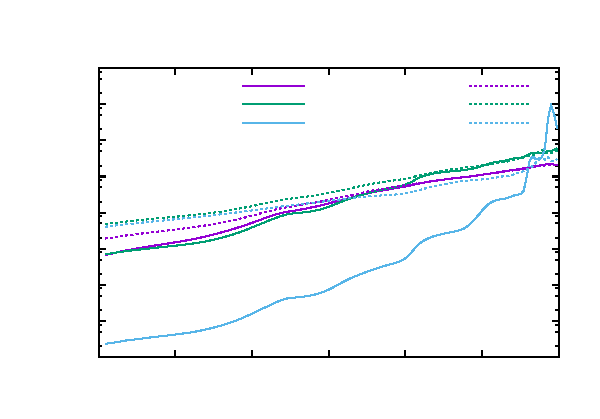
\includegraphics{cosA_distrib-G-250km-90deg}}%
    \gplfronttext
  \end{picture}%
\endgroup
